\documentclass[a4paper,12pt]{article}
\usepackage{graphicx}
\usepackage{amsmath}
\usepackage{amsthm}
\usepackage{amssymb} 
\usepackage[hidelinks]{hyperref} % Add hidelinks to suppress link boxes
\usepackage{enumitem}
\usepackage{geometry}
\usepackage{tocloft}
\usepackage{graphicx}
\usepackage{float,graphicx}
\usepackage{xcolor}

% new functions
\theoremstyle{definition}
\newtheorem{example}{Example}

\numberwithin{equation}{section}
\numberwithin{figure}{section}
\numberwithin{example}{subsection}

% Geometry Settings
\geometry{margin=1in}

% Header and Footer
\usepackage{fancyhdr}
\pagestyle{fancy}
\fancyhf{}
\fancyhead[L]{STA414}
\fancyfoot[R]{\thepage}

% Title
\title{STA414: Statistical Methods for Machine Learning II \\ Lecture Notes}
\author{Yiliu Cao}
\date{May 3, 2024}

% Table of Contents Settings
\renewcommand{\cftsecleader}{\cftdotfill{\cftdotsep}}
\setcounter{tocdepth}{2}

\begin{document}

% Title Page
\maketitle
\thispagestyle{empty}

% Table of Contents
\tableofcontents
\newpage

%-------------1: Probabilistic models-----------
\section{Probabilistic models}
\subsection{An overview of probabilistic models}
\label{sec:pro-models}
We have the random vector $X=(X_1,X_2,\cdots X_n)$, and we want to compute the relationship between each random variable. The joint distribution is $p(x)=p(x_1,\cdots,x_d)$. Denote the input data \textbf{x} (high-dimensional), and output y (discrete or continuous). In general, we have two models:\\
\newline
\textbf{Regression}: $$p(y | x) = \frac{p(x,y)}{p(x)}=\frac{p(x,y)}{\int p(x,y) \, dy}$$\\
\textbf{Classification/Clustering}: $$p(c | x) = \frac{p(x,c)}{\sum_{c} p(x,c)}$$

\subsection*{Observed vs Unobserved random variables}
\textbf{Supervised classification(learning)}:
\begin{itemize}
    \item We \textbf{KNOW} what to predict
    \item \textbf{Supervised Dataset:} $\{x^{(i)}, c^{(i)}\}_{i=1}^N \sim p(x, c)$
    \item The class labels are observed.
\end{itemize}
\textbf{Unsupervised classification(learning)}:
\begin{itemize}
    \item We do \textbf{NOT KNOW} what to predict
    \item \textbf{Unsupervised Dataset:} $\{x^{(i)}\}_{i=1}^N \sim p(x) = \sum_c p(x,c)$
    \item We only observe the inputs \textbf{x}
\end{itemize}
In order to estimate the unknown distribution $p(x)$, we have few assumptions:
\begin{enumerate}
    \item \textbf{IID Data}: we assume the samples $x^{(i)}$ are independent and identically distributed.
    \item \textbf{Parametrized distribution}: $p(x|\theta)$ comes from a parametrized family $\mathcal{P} = \left\{ p(x | \theta) : \theta \in \Theta \right\}$
\end{enumerate}

\subsection*{Maximum Likelihood Estimation(MLE)}
MLE is the method to estimate the parameters of an assume probability distribution, given some observed data. Technically, we can use MLE to estimate any parameters we want. More specifically:
\begin{itemize}
    \item Let $x^{(i)} \sim {p_*} = p(x | \theta_*)$ for $i = 1, \ldots, N$ be i.i.d. random variables.
    \item The joint of $\mathcal{D} = \{ x^{(1)}, x^{(2)}, \ldots, x^{(N)} \}$ is $p(\mathcal{D} | \theta_*) = \prod_{i} p(x^{(i)} | \theta_*)$.
    \item Assume we observe data $\mathcal{D}$ and $\theta_*$ is unknown. The likelihood function is:
    $$
    \mathcal{L}(\theta; \mathcal{D}) = p(\mathcal{D} | \theta) = \prod_{i=1}^{N} p(x^{(i)} | \theta)
    $$
    \item The log-likelihood function:
    $$
    \ell(\theta; \mathcal{D}) = \log \mathcal{L}(\theta; \mathcal{D}) = \sum_{i=1}^{N} \log p(x^{(i)} | \theta)
    $$
\end{itemize}
Here is an \hyperref[example-1]{example} of MLE
\subsection*{Sufficient Statistics and Exponential Families}
A \textbf{sufficient statistics} is a function of the data that conveys exactly the same information about the parameter as the entire data.\\
In addition, we can writing any exponential family member in the form:
$$p(x | \eta) = h(x) \exp \{ \eta^{\top} T(x) - A(\eta) \}$$
where
\begin{align*}
    T(x) &: \text{sufficient statistics} \\
    \eta &: \text{natural parameter} \\
    A(\eta) &: \text{log-partition function} \\
    h(x) &: \text{carrying measure}
\end{align*}
Moreover, let $X\sim p(x|\eta)$, then we have $E[T(X)]=A^\prime(\eta)$\\
One \hyperref[example-2]{example} of exponential family

\subsection{Statistical decision theory}
Suppose we have an input vector $x$ and the corresponding target, we want to predict the label given a new input. Notice that here we assume the output is the label/class which is discrete. However, the output can also be continuous (regression).\\
\newline
Intuitively, for a given new input $x$, we have:
$$p(\mathcal{C}_k| x)=\frac{p(x|\mathcal{C}_k)p(\mathcal{C}_k)}{p(x)}$$
We then pick the $\mathcal{C}_k$ with the highest probability.\\
\textbf{Decision Rule}: Divide the input space to $\mathcal{R}_1\:\&\:\mathcal{R}_2$ such that all points in $\mathcal{R}_k$ are assigned to class $\mathcal{C}_k$. We want to make mistakes as less as possible; equivalently, we want to minimize the \textbf{misclassification rate}.\\
For $k\in\{1,\:2\}$:
\begin{align}
p(\text{mistake})&=p(x\in\mathcal{R}_2,\:\mathcal{C}_1)+p(x\in\mathcal{R}_2,\:\mathcal{C}_1)=\int_{\mathcal{R}_{1}} p\left(x, \mathcal{C}_{2}\right) d x+\int_{\mathcal{R}_{2}} p\left(x, \mathcal{C}_{1}\right) dx
\end{align}


\begin{figure}
    \centering
    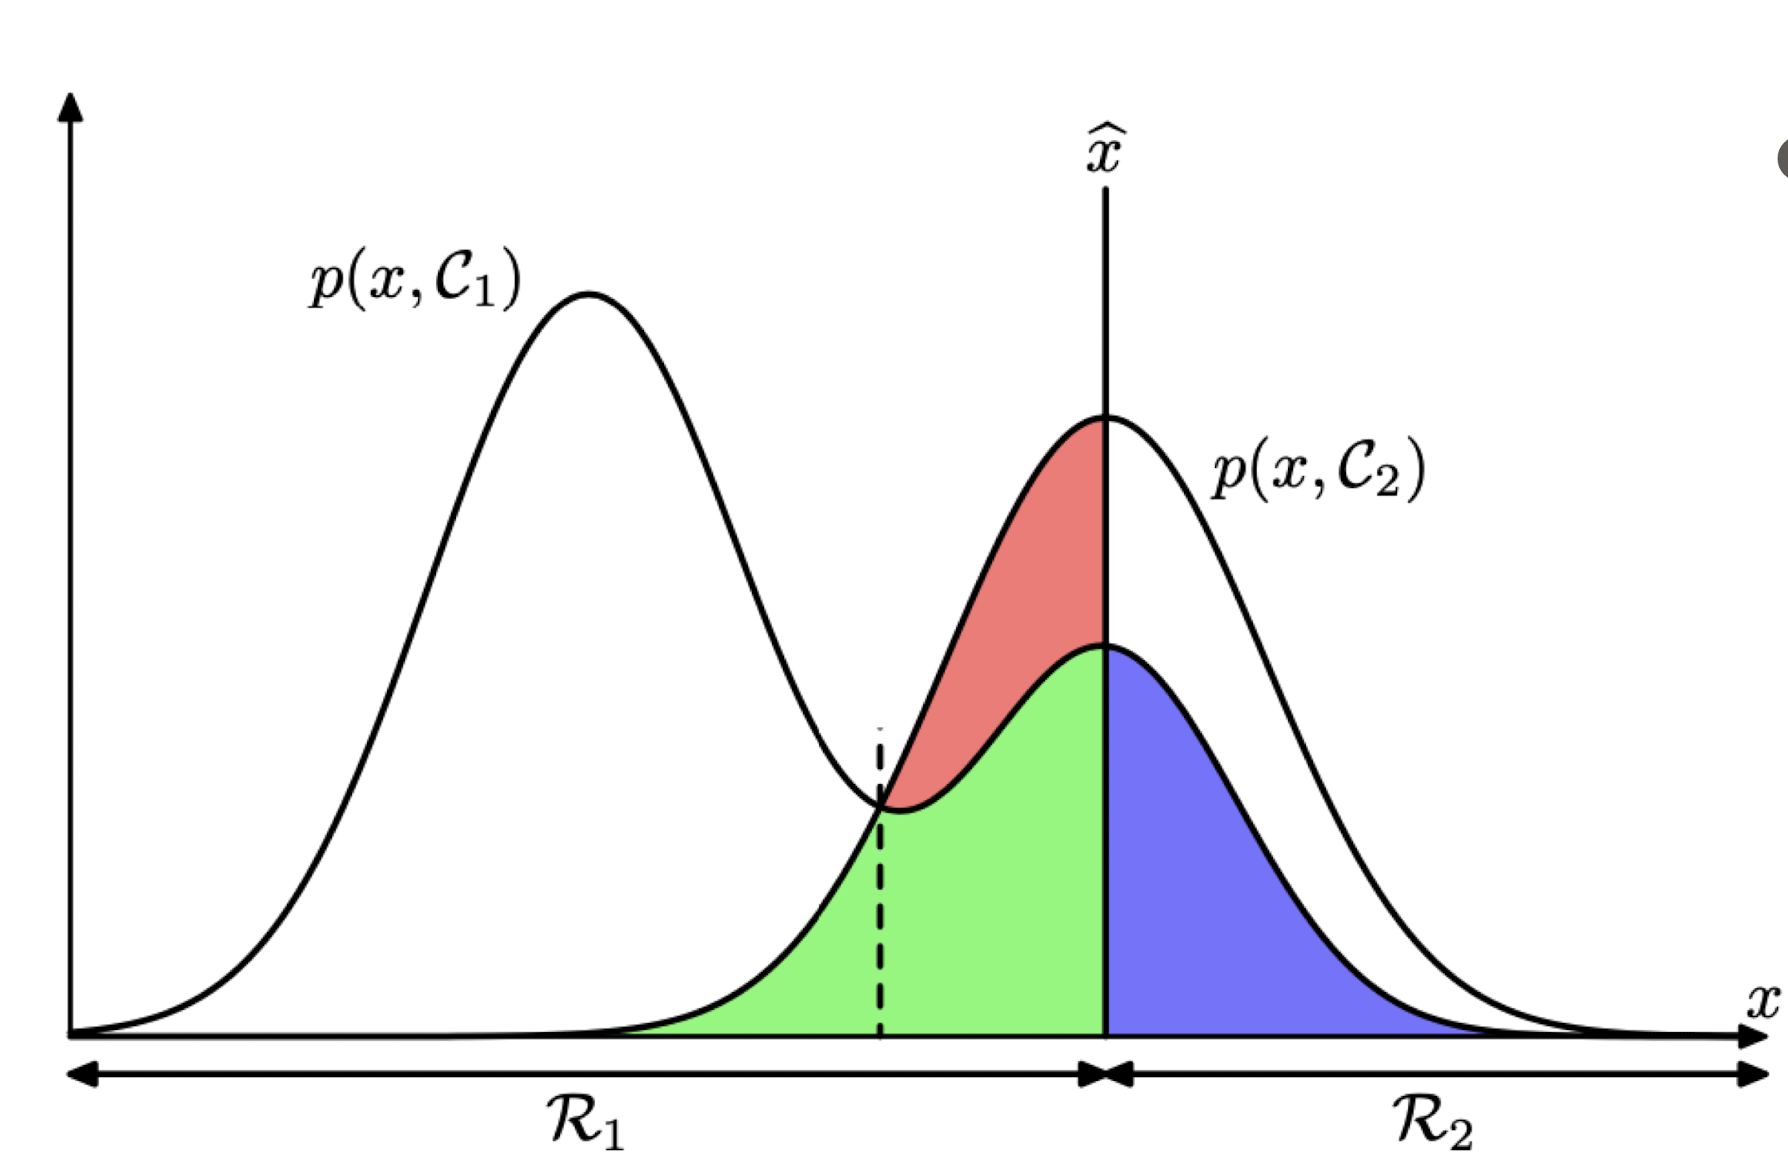
\includegraphics[width=.7\linewidth]{figure_1.png}
    \caption{Misclassification Rate}
    \label{fig:my_label}
\end{figure}
\begin{enumerate}
    \item \textbf{RedGreen regions}: inputs that belong to $\mathcal{C}_2$ but assigns to $\mathcal{R}_1$ as they are under $ p\left(x, \mathcal{C}_{2}\right)$.
    \item \textbf{Blue regions}: inputs that belong to $\mathcal{C}_1$ but assigns to $\mathcal{R}_2$ as they are under $ p\left(x, \mathcal{C}_{1}\right)$
    \item Therefore, for any data \textbf{x}, if $ p\left(x, \mathcal{C}_{1}\right)>p\left(x, \mathcal{C}_{2}\right)$, then we assign this point to $\mathcal{C}_1$, vice-versa. Therefore, $\mathcal{R}=\{x:\:p\left(x, \mathcal{C}_{1}\right)>p\left(x, \mathcal{C}_{2}\right)\}$
\end{enumerate}
We want to minimize the misclassification error rate $\Rightarrow$ minimize the \textbf{loss}
\subsection*{Loss Function} 
\textbf{Loss function} measures the loss incurred by taking of any available decisions. 
\subsubsection*{For discrete case}
we denote $L_{ij}$ as the $(k,\:j)$ element of the loss matrix. We want to minimize the expected loss\\
Therefore:
\begin{align*}
\mathbb{E}[L] & =\sum_k \sum_j \int_{\mathcal{R}_j} L_{k j} p\left(x, \mathcal{C}_k\right) d x\\
& =\sum_j \int_{\mathcal{R}_j} \sum_k L_{k j} p\left(x, \mathcal{C}_k\right) d x
\end{align*}
Define $g_j(x)=\sum_k L_{k j} p\left(x, \mathcal{C}_k\right)$. Notice that $g_j(x) \geq 0$ and
$$\mathbb{E}[L]=\sum_j \int_{\mathcal{R}_j} g_j(x) d x$$
Thus, minimizing $\mathbb{E}[L]$ is equivalent to choosing
\begin{align}
    \mathcal{R}_j&=\left\{x: g_j(x)<g_i(x) \text { for all } i \neq j\right\}\\
    \Rightarrow \mathcal{R}_j &=\left\{x: \sum_k L_{k j} p\left(\mathcal{C}_k \mid x\right)<\sum_k L_{k i} p\left(\mathcal{C}_k \mid x\right) \text { for all } i \neq j\right\}
\end{align}
\subsubsection*{For regression}
\begin{itemize}
    \item Consider the input/target $(x,\:t)$, where $t$ is continuous and the joint density is $p(x,\:t)$
    \item The regression function is $y(t)$
    \item The loss function is $L(y(x),\:t)=(y(x)-t)^2$
\end{itemize}
Therefore the expected loss will be:
\begin{align*}
\mathbb{E}[L]&=\iint L(y(x), t) p(x, t) d x d t\\
&=\iint(y(x)-\mathbb{E}[t \mid x])^2 p(x, t) d x d t+\iint(\mathbb{E}[t \mid x]-t)^2 p(x, t) d x dt
\end{align*}
Full derivations \hyperref[derivations-1]{here}\\
The second term is the conditional variance of $t|x$ and does not depend on $y(x)$ and hence the expected loss is minimized when $y(x)=\mathbb{E}[t|x]$. Therefore, we can see that the loss function will change the decision rule significantly; however, we can always reject the option or not making a decision.


%-------------2: Graphical models-----------
\section{Graphical Models}
\label{sec:graphical-models}

\subsection{Introduction to graphical models}
Remember our goal is to specify the joint distribution \textit{N} random variables $p(x_1,\cdots,x_N)=p(x)$. If we assume each $x_i$ is binary such that $x_i\in\{0,\:1\}$, then we need $\mathbf{2^N-1}$ parameters to specify $p(x)$. For example, $p(x_1=0,\:x_2=0,\:\cdots,x_N=0)\:\text{or}\:p(x_1=1,\:x_2=0,\:\cdots,x_N=0)$.\\ Equivalently, we can specify the joint distribution $p(x)$ as:
\begin{align*}
    p\left(x_1, x_2, \ldots, x_N\right)&=\prod_{j=1}^N p\left(x_j \mid x_1, x_2, \ldots, x_{j-1}\right)\\
    &=p(x_1|x_0)p(x_2|x_1,\:x_0)\cdots
\end{align*}
Thus total number of parameters is $1+2+4+\cdots2^{N-1}=2^N-1$\\
We can see that it requires a huge number of parameters to specify the joint distribution. We want to draw relationships between variables.
\subsubsection*{Condition independence}
For three random variables $x_A,\:x_B\:x_C$, if $x_A,\:x_B$ are conditionally independent given $x_C$, then we write $x_A\perp x_B\mid x_C$. The following conditions are equivalent:
\begin{itemize}
    \item $x_A\perp x_B\mid x_C$
    \item $p(x_A,\:x_B|x_C)=p(x_A|x_C)p(x_B|x_C)$
    \item $p(x_A|x_B,\:x_C)=p(x_A|x_C)$
    \item $p(x_B|x_A,\:x_C)=p(x_B|x_C)$
\end{itemize}
\subsection{Directed Acyclic Graphical Models}
A directed cyclic graphical model encode a particular form of factorization of the joint distribution. The form of factorization is various.\\
\begin{figure}
    \centering
    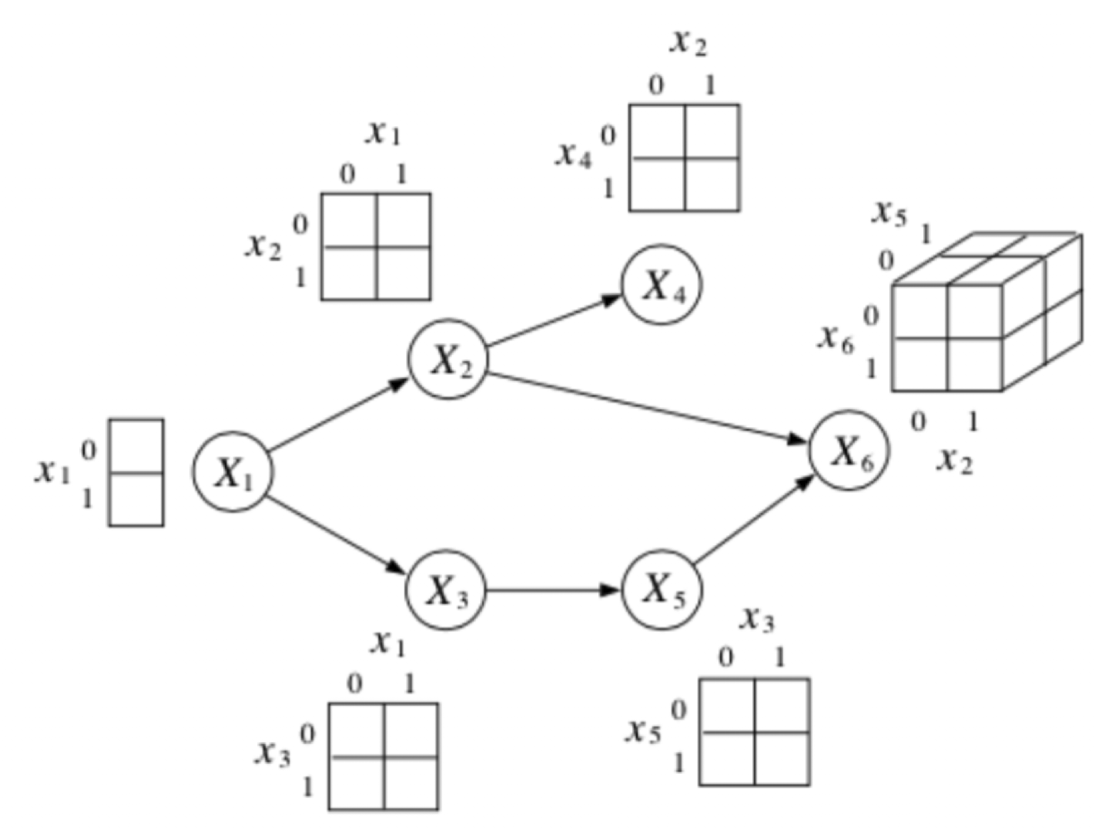
\includegraphics[width=.7\linewidth]{codes/figures/section2/figure_2_1.png}
    \caption{An example of conditional probability tables(CPT)}
    \label{fig:figure_2}
\end{figure}
\hyperref[fig:figure_2]{Figure 2} shows an example of conditional probability. From the graph, we only need $2^1*4+2^0+2^2=13<2^6-1$ parameters.\\
\textbf{D-separation}: If $C$ d-separates $A$ and $B$, then $x_A\perp x_B\mid x_C\:\forall a\in A,\:b\in B$
\subsubsection*{Bayes ball algorithm}
Bayes ball determines the conditional independence/dependence in a DAG (I personally found this part most ambiguous). There are three fundamental Bayes ball algorithms which are causal chain, common cause and explaining away. For each one, we will under it intuitively by drawing a story.
\begin{enumerate}
  \item \textbf{Causal chain}

  \begin{figure}[H]
    \centering
    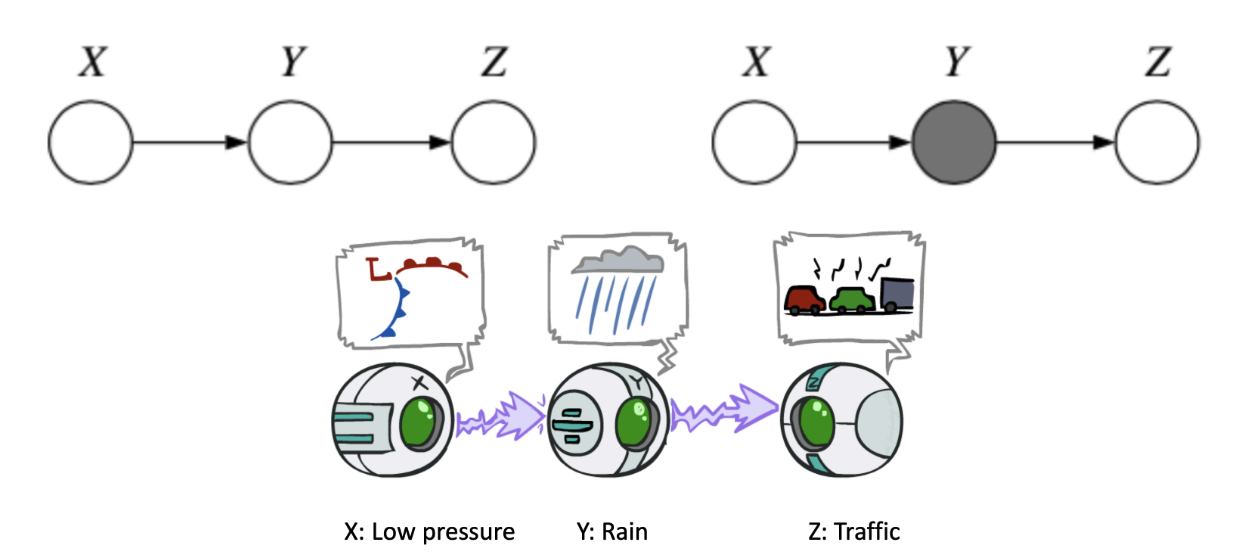
\includegraphics[width = .7\linewidth]{codes/figures/section2/figure_2_2.png}
    \caption{An illustration of causal chain}
  \end{figure}
  \begin{align*}
    p(z \mid x, y) & =\frac{p(x, y, z)}{p(x, y)} \\
    & =\frac{p(x) p(y \mid x) p(z \mid y)}{p(x) p(y \mid x)} \\
    & =p(z \mid y) \quad \\
    \Rightarrow X\text { and }& Z \text { d-separated given } Y
  \end{align*}
  
  \item \textbf{Common cause}

  \begin{figure}[H]
    \centering
    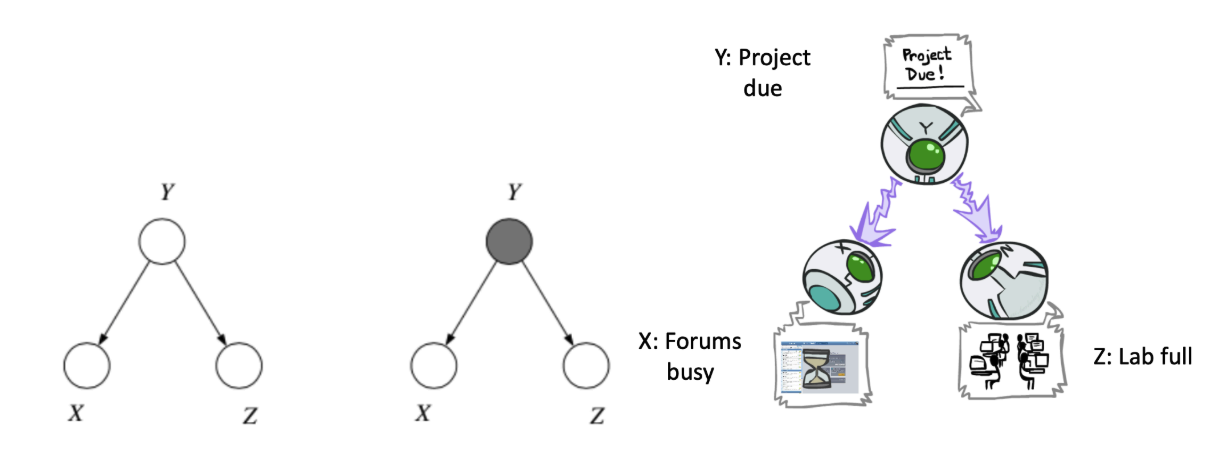
\includegraphics[width = .7\linewidth]{codes/figures/section2/figure_2_3.png}
    \caption{An illustration of common cause}
  \end{figure}
  \begin{align*}
    p(x, z \mid y)&=\frac{p(x, y, z)}{p(y)}\\
    &=\frac{p(y) p(x \mid y) p(z \mid y)}{p(y)}\\
    &=p(x \mid y) p(z \mid y)\\
    \Rightarrow X\text { and }& Z \text { d-separated given } Y
  \end{align*}
  
  \item \textbf{Explaining away}

  \begin{figure}[H]
    \centering
    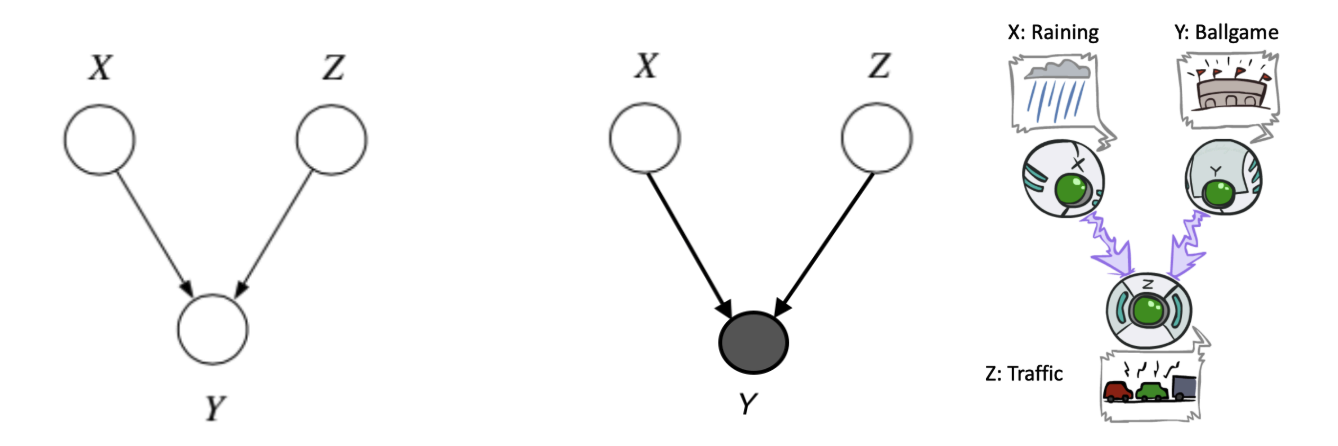
\includegraphics[width = .7\linewidth]{codes/figures/section2/figure_2_4.png}
    \caption{An illustration of explaining away}
  \end{figure}
  \begin{align*}
    p(z \mid x, y) & =\frac{p(x) p(z) p(y \mid x, z)}{p(x) p(y \mid x)} \\
    & =\frac{p(z) p(y \mid x, z)}{p(y \mid x)} \neq p(z \mid y)\\
    \Rightarrow X\text { and }& Z \text { are NOT d-separated given } Y
  \end{align*}
\end{enumerate}
In general, the Bayes ball works as follows:
\begin{enumerate}
    \item Shade all nodes $x_C$ (these are observed)
    \item Place "balls" at each node in $x_A$ (or $x_B$ )
    \item Let the "balls" "bounce" around according to some rules. If any of the balls reach any of the nodes in $x_B$ from $x_A$ then $x_A \not\perp x_B \mid x_C$. Otherwise $x_A \perp x_B \mid x_C$
\end{enumerate}
\textbf{Example}\\
\textit{Question:} Is $x_2\perp x_3\mid\{x_1,\:x_6\}$
\begin{figure}[H]
    \centering
    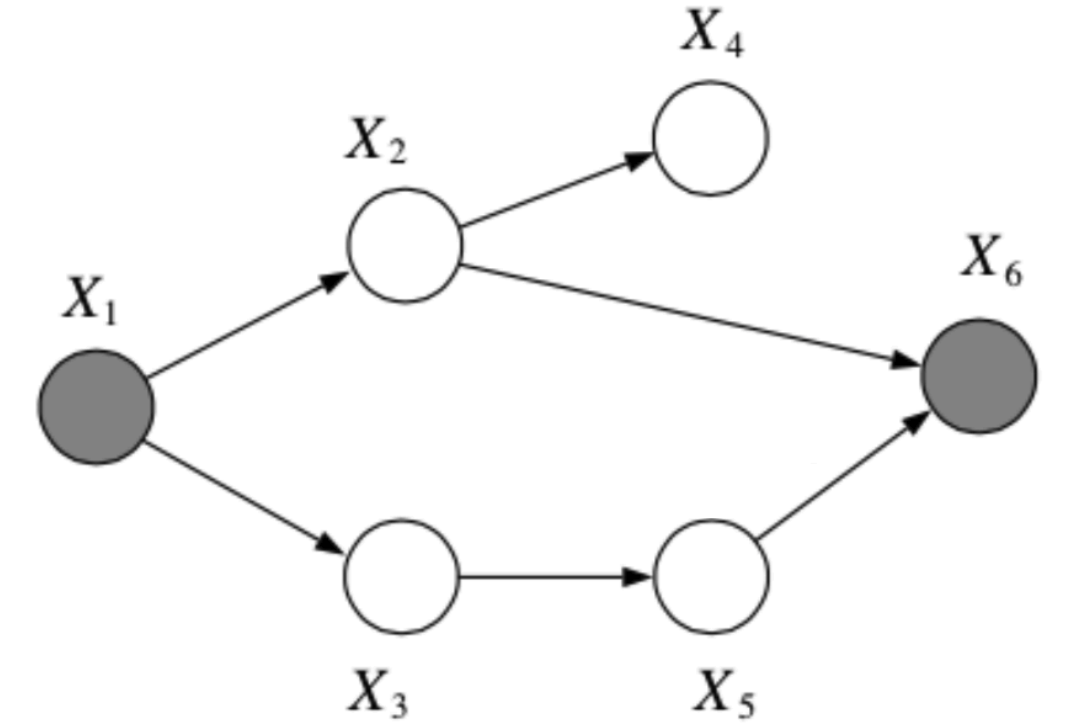
\includegraphics[width = .7\linewidth]{codes/figures/section2/figure_2_5.png}
    \caption{An illustration of explaining away}
\end{figure}
\textit{Answer:} No. By Bayes ball algorithm, $x_2$ can travel to $x_5$, and hence can travel to $x_3$.
\subsubsection*{Moralization}
Like I said, I personally do not like Bayes algorithm. Instead, another one called "moralization" is more straightforward and easier to use. We can follow the procedure:
\begin{enumerate}
    \item \textbf{Draw the ancestral graph}\\
    We only keep the ancestor of the mentioned nodes. That said, in the previous example, we only keep the ancestors of $\{x_2,\:x_3,\:x_1\:x_6\}$. Hence we have the entire graph except the node $x_4$. Note the ancestors includes \textbf{their parents, parents' parents etc}.
    \item \textbf{"Moralize" the ancestral graph by "marrying" the parents}\\
    If two nodes have the same children, such as $x_2$ and $x_5$, then we draw a line between these two nodes.
    \item \textbf{"Disorient" the graph}\\
    Ignore the directions by replacing the arrows to edges.
    \item \textbf{Delete the givens and their edges}\\
    In the previous example, the givens are the $x_1$ and $x_4$.
    \item \textbf{Find the answer}\\
    After we finished the step 1 to 4, we then justify whether the two nodes are connected or disconnected. If \textbf{connected}, then the two nodes are conditionally \textbf{dependent}. Otherwise \textbf{disconnected}, the two nodes are conditionally \textbf{independent}. In the previous example, we can easily find that $x_2$ and $x_3$ are d-separated by $x_1$ and $x_6$.
\end{enumerate}
\textit{Question}: What about the marginal independence, such as $x_2\perp x_3$?\\
\textit{Answer}: We use the same way as above without step 4.

\subsection{Undirected Graphical Models}
The undirected graphical models are also called the \textbf{Markov random fields (MRFs)}. Compare to graphical models, we have no more directed edges; instead, the dependencies are now described as undirected graphs. Moreover, \textbf{Markov blanket} is the set of nodes that makes $X_i$ conditionally independent of all other nodes. \textbf{Clique} is a subset of nodes that every two nodes are connected by an edge. \textbf{Maximal clique} a clique that can not be extended by including one more adjacent vertex.
\begin{figure}[H]
    \centering
    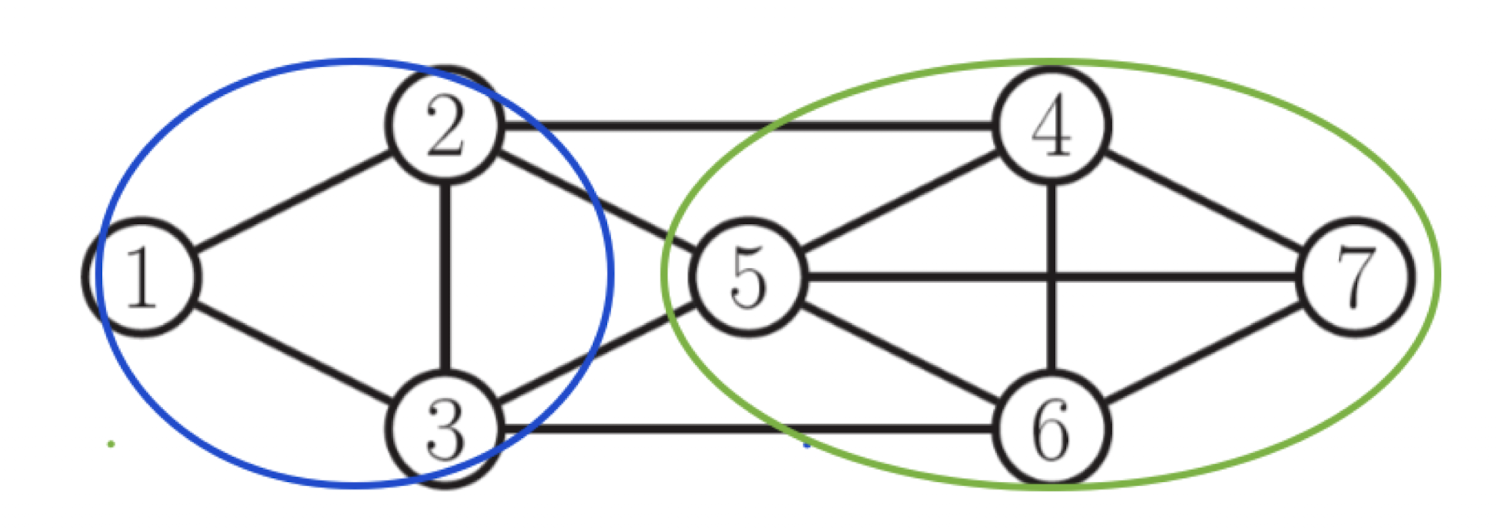
\includegraphics[width = .7\linewidth]{codes/figures/section2/figure_2_6.png}
    \caption{An example of Markov random fields: \{1, 2, 3\} is a clique and \{4, 5, 6, 7\} is a maximal clique}
    \label{fig:mrf}
\end{figure}
\subsubsection*{Distribution induced by MRFs}
\begin{itemize}
    \item Let $X=\left(X_1, \ldots, X_m\right)$ be the set of all random variables in our graph $G$.
    \item Let $\mathcal{C}$ be the set of all maximal cliques of $G$.
    \item The distribution $p$ of $X$ factorizes with respect to $G$ if
$$
p(x) \propto \prod_{C \in \mathcal{C}} \psi_{\mathcal{C}}\left(x_C\right)
$$
for some nonnegative potential functions $\psi_C$, where $x_C=\left(x_i\right)_{i \in C}$.
\end{itemize}
The density can be factorized to cliques is also called the \textbf{Hammersley-Clifford Theorem}.\\
\textbf{Global markov properties}: $X_A\perp X_B\mid X_S$ if the sets $A$ and $B$ are separated by $S$ in $G$ (every path from $A$ to $B$ has to pass $S$).
Therefore, the joint distribution described on \hyperlink{fig:mrf}{above} is: 
\begin{align*}
  p(x) \propto & \psi_{1,2,3}\left(x_1, x_2, x_3\right) \psi_{2,3,5}\left(x_2, x_3, x_5\right) \psi_{2,4,5}\left(x_2, x_4, x_5\right) \\
  & \times \psi_{3,5,6}\left(x_3, x_5, x_6\right) \psi_{4,5,6,7}\left(x_4, x_5, x_6, x_7\right)
  \end{align*}
\colorbox{yellow}{Not all DAGMs can be represented as MRFs.}.\\
\subsubsection*{Relations between exponential families and MRFs}
\begin{itemize}
  \item Consider a parametric family of factorized distributions
  $$
  p(x \mid \theta)=\frac{1}{Z(\theta)} \prod_{C \in \mathcal{C}} \psi_c\left(x_C \mid \theta_C\right), \quad \theta=\left(\theta_C\right)_{c \in \mathcal{C}} .
  $$
  \item We can write this in an exponential form:
  $$
  p(x \mid \theta)=\exp \{\sum_{C \in \mathcal{C}} \log \psi_C\left(x_C \mid \theta_C\right)-\underbrace{\log Z(\theta)}_{=A(\theta)}\}
  $$
  \item Suppose the potentials have a log-linear form
  $$
  \log \psi_C\left(x_C \mid \theta_C\right)=\theta_C^{\top} \phi_C\left(x_C\right)
  $$
  we then get the exponential family
  $$
  p(x \mid \theta)=\exp \{\sum_{C \in \mathcal{C}} \theta_C^{\top} \phi_C\left(x_C\right)-\underbrace{\log Z(\theta)}_{=A(\theta)}\}
  $$
\end{itemize}
\textit{Question}: When the potentials have a log-linear form?\\
\textit{Solution}: Suppose we have the random vector $x_1$ and $x_2$, and they are all binary. Then there are four possible values of $(x_1,\:x_2)$: (0, 0), (1, 0), (0, 1), (1, 1). We take\\
$$
\theta_{1,2}:=\left[\begin{array}{l}
\log \psi_{1,2}(0,0) \\
\log \psi_{1,2}(0,1) \\
\log \psi_{1,2}(1,0) \\
\log \psi_{1,2}(1,1)
\end{array}\right] \in \mathbb{R}^4
$$
and let $\psi_{1,2}\left(x_1, x_2\right)$ be the function that satisfies
$$
\phi_{1,2}(0,0)=\left[\begin{array}{l}
1 \\
0 \\
0 \\
0
\end{array}\right], \quad \phi_{1,2}(0,1)=\left[\begin{array}{l}
0 \\
1 \\
0 \\
0
\end{array}\right], \quad \phi_{1,2}(1,0)=\left[\begin{array}{l}
0 \\
0 \\
1 \\
0
\end{array}\right], \quad \phi_{1,2}(1,1)=\left[\begin{array}{l}
0 \\
0 \\
0 \\
1
\end{array}\right].
$$

$$\Rightarrow\phi_{1,2}\left(x_1, x_2\right)=\left[\begin{array}{c}
  \left(1-x_1\right)\left(1-x_2\right) \\
  \left(1-x_1\right) x_2 \\
  x_1\left(1-x_2\right) \\
  x_1 x_2
  \end{array}\right]
$$
We then have a linear form:$$
\log \psi_C\left(x_{12} \mid \theta_{12}\right)=\theta_{12}^{\top} \phi_{12}\left(x_{12}\right)
$$
\subsubsection*{Ising model}
The Ising model is an example of MRFs, which is used to model magnets. It has a form of potential function:
$$\psi_{st}(x_s,\:x_t)=e^{J_{st}x_sx_t}$$
Equivalently:
$$\psi_{st}(-1,\:-1)=\psi_{st}(1,\:1)=e^{J_{st}}$$
$$\psi_{st}(1,\:-1)=\psi_{st}(-1,\:1)=e^{-J_{st}}$$
$$\psi_{st}(x_s,\:x_t)=0\:\text{if the two nodes are not connected}$$
In terms of the distribution in Ising model, we also incldue the node potential $\psi_s(x_s)=e^{b_sx_s}$:
$$p(x) \propto \prod_{s \sim t} \psi_{s t}\left(x_s, x_s\right) \prod_s \psi_s\left(x_s\right)=\exp \left\{\sum_{s \sim t} J_{s t} x_s x_t+\sum_s b_s x_s\right\}$$
\textbf{Recall: Multivariate normal distribution}\\
$X=\left(X_1, \ldots, X_m\right): \mu \in \mathbb{R}^m$ and $\Sigma$ symmetric positive definite $m \times m$ matrix. Write $X \sim N_m(\mu, \Sigma)$ if the density of the vector $X$ is
$$
f(\boldsymbol{x} ; \mu, \Sigma)=\frac{1}{(2 \pi)^{m / 2}}(\operatorname{det} \Sigma)^{-1 / 2} \exp \left(-\frac{1}{2}(\boldsymbol{x}-\mu)^T \Sigma^{-1}(\boldsymbol{x}-\mu)\right) .
$$
Denote $K=\Sigma^{-1}$ then
$$
f(\boldsymbol{x} ; \mu, \Sigma) \propto \prod_{\boldsymbol{s}} e^{-\frac{1}{2} K_{s s}\left(x_s-\mu_s\right)^2} \prod_{\boldsymbol{s}<t} e^{-K_{s t}\left(x_s-\mu_s\right)\left(x_t-\mu_t\right)}
$$
Intuitively, we can also visualize the conditional independencies between each variables (similar to Bayes ball). Just like the Ising model, here we can use concentration matrix $K$ to represent the relationship between variables.\\
Conditional independence:
\begin{itemize}
  \item $X_i \perp X_j$ if and only if $\Sigma_{i j}=0$.
  \item $X_i \perp X_j \mid X_C \quad$ if and only if $\quad \Sigma_{i j}-\Sigma_{i, C} \Sigma_{C, C}^{-1} \Sigma_{C, j}=0$
  \item Let $R=V \backslash\{i, j\}$. The following are equivalent:
  \begin{itemize}
    \item $X_i \perp X_j \mid X_R$
  \item $\Sigma_{i j}-\Sigma_{i, R} \Sigma_{R, R}^{-1} \Sigma_{R, j}=0$
  \item $\left(\Sigma^{-1}\right)_{i j}=0$ 
  \end{itemize}
\end{itemize}
Hence we have the \textbf{Gaussian Graphical models}
\begin{figure}[H]
  \centering
  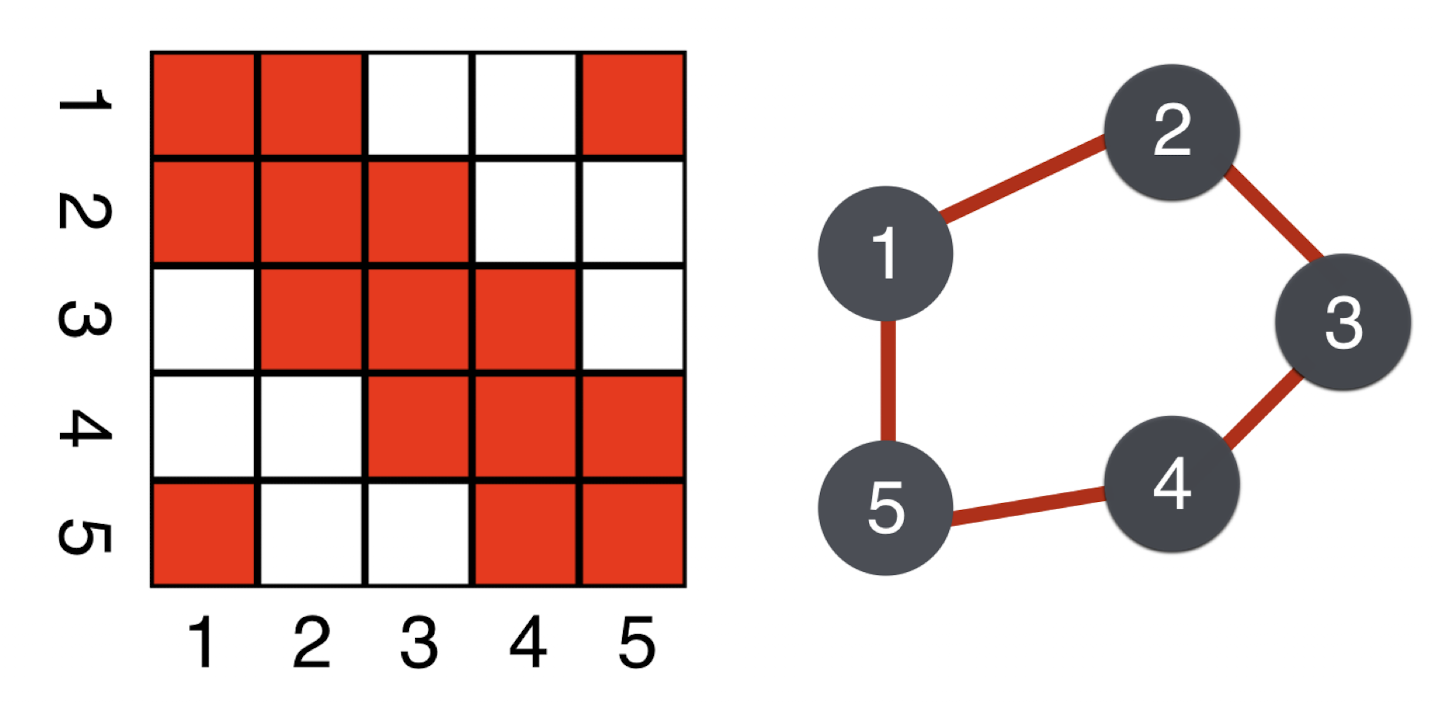
\includegraphics[width = .7\linewidth]{codes/figures/section2/figure_2_7.png}
  \caption{An example of Gaussian Graphical model}
  \label{fig:ggm}
\end{figure}
$K_{ij}=0$ if and only if $X_i\perp X_j\mid X_{rest}$. For example, $X_1\perp X_4\mid X_{rest}$

%-------------3: Inference-----------
\section{Inference}
\subsection{Introduction to statistical inference}
We want to explore the inference from the probabilistic graphical models. In notations, we have
\begin{itemize}
    \item $x_E$ represent the observed evidence
    \item $x_F$ represent the unobserved varaible we want to infer
    \item $x_R=x\{x_E,\:x_F\}$ represent the remaining variables
\end{itemize} 
For the conditional probability $p(x_F|x_E)$, by Bayes theorem:
$$p\left(x_F \mid x_E\right)=\frac{p\left(x_F, x_E\right)}{p\left(x_E\right)}=\frac{p\left(x_F, x_E\right)}{\sum_{x_F} p\left(x_F, x_E\right)}$$
Moreover, we can also marginalize the extraneous variables to have the marginal joint distribution:
$$p\left(x_F, x_E\right)=\sum_{x_R} p\left(x_F, x_E, x_R\right)$$
The below equation give us an intuition of exact inference, which is to marginalize other variables. However, when the number of variables increases, the order we marginalize will affect the computational cost. Hence we have to choose an appropriate \textbf{elimination order}. More specifically, we want to have the exact inference for one variable in DAGMs or MRFs.
\begin{example}
    \text{Suppose we have the simple chain for four variables A, B, C, D}\\
    $$A \rightarrow B \rightarrow C \rightarrow D$$
    where:
    $$x_F=\{D\},\:x_E=\{A,\:B,\:C\},\:x_R=\{\}$$
    We want to compute the exact inference of $D$, $p(D)$
    In the simple chain settings, we can express the joint distribution as:
    \begin{align*}
        p(D)&=\sum_{A,B,C}p(A,B,C,D)\\
        &=\sum_C \sum_B \sum_A p(A) p(B \mid A) p(C \mid B) p(D \mid C)
    \end{align*}
    If we choose an elimination order:
    \begin{align*}
        p(D)&=\sum_{A,B,C}p(A,B,C,D)\\
        &=\sum_C p(D \mid C)\left(\sum_B p(C \mid B)\left(\sum_A p(A) p(B \mid A)\right)\right)\\
        &=\sum_C p(D \mid C) \sum_B p(C \mid B) \sum_A p(A) p(B \mid A) \\
        & =\sum_C p(D \mid C) \sum_B p(C \mid B) p(B) \\
        & =\sum_C p(D \mid C) p(C)\\
        & =\sum_C p(D,\:C)
    \end{align*}
\end{example}
The above example give us an intuition that we can firstly marginalize the node with no children ($C$ first). Equivalently, we start the nodes that comes early in the induced ordering of the DAG.
\subsection{Sum-product algorithm}
\begin{example}
    ss
\end{example}

%-------------4: Message Passing-----------
\section{Message passing}
\label{sec:message-passing}
\subsection{TrueSkill latent variable models}
\textbf{Latent variables} are variables that can only be inferred indirectly through a mathematical model from other observable variables that can be directly observed or measured.\\
\newline
\textbf{TrueSkill} model is a player ranking system for competitive games. Our goal is to infer the skills of players in a competitive game, based on the results of the games. Hence, each player's skill is a \textbf{latent variable}, and we assume they are fixed. Moreover, we also assume each player's skill is independent such as independent Gaussian prior.\\
\newline
For each game, the probability that player $i$ beats player $j$ is
$$p(i\:\text{beats}\:j)=\sigma(z_i-z_j),\:\text{where}$$
$$\sigma{(y)}=\frac{1}{1+\text{exp}(-y)}$$
Hence the entire joint likelihood of players and games is:
\begin{gather*}
    p\left(z_1, z_2, \ldots z_N, \text { game } 1, \text { game } 2, . . \text { game } T\right) \\
    =\underbrace{\left[\prod_{i=1}^N p\left(z_i\right)\right]}_{\text{prior}} \underbrace{\left[\prod_{\text {games }} p\left(\mathrm{i} \text { beats } \mathrm{j} \mid z_i, z_j\right)\right]}_{\text{likelihood}}
\end{gather*}
However, it is hard to compute the posterior
\begin{align*}
    & p\left(z_1, z_2 \mid \text { game } 1 \text {, game } 2, \ldots \text { game } T\right) \\
    = & \int \cdots \int p\left(z_1, z_2, z_3 \ldots z_N \mid x\right) d z_3 \ldots d z_N
\end{align*}
\textbf{Message passing} can help us to compute the posterior.

\subsection{Message Passing}
From the last section, we can see that determining an optimal elimination order is hard, and the resulting marginalization can be still costly. Therefore, we introduce the tress as any elimination ordering from leaves to the root is optimal.
\subsubsection*{Inference in trees}
A graph is $G=(\mathcal{V},\:\mathcal{E})$, where $\mathcal{V}$ is vertices and $\mathcal{E}$ is edges. A leaf in a tree is the nodes where it has only one neighbor. We can regard a tress as MRFs, with joint distribution:
$$p\left(x_1, x_2, \ldots, x_n\right)=\underbrace{\frac{1}{Z}}_{\text{normalization}}\overbrace{\prod_{i \in \mathcal{V}} \psi\left(x_i\right)}^{\text{nodes}}\underbrace{\prod_{(i, j) \in \mathcal{E}} \psi_{i j}\left(x_i, x_j\right)}_{\text{edges}}$$
\begin{example}
    \begin{figure}[H]
        \centering
        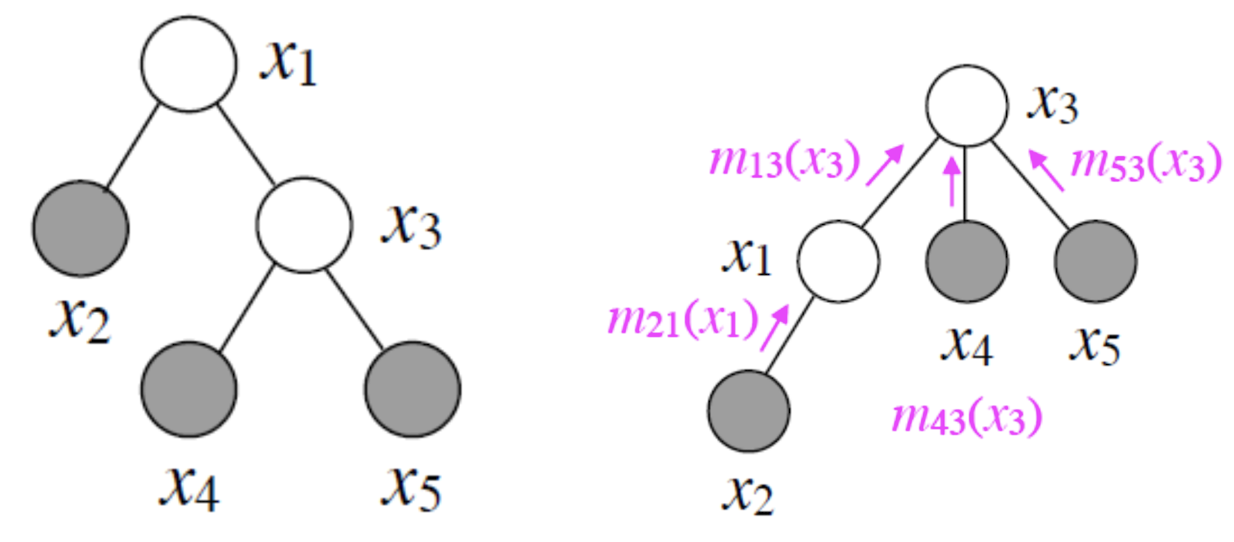
\includegraphics[width = .6\linewidth]{codes/figures/section4/figure_4_1.png}
        \caption{An example of tree and message passing}
        \label{fig:tree}
    \end{figure}
    \hyperref[fig:tree]{Above} shows a tree where $x_E=\{\bar{x_2},\bar{x_4},\bar{x_5}\},\:x_R=x_1$. We want to compute $p(x_3\mid x_E)$:
    \begin{align*}
        p(x_3|x_E)&=\frac{p\left(x_3, x_E\right)}{\sum_{x_3^{\prime}} p\left(x_3^{\prime}, x_E\right)}\\
        &=\frac{1}{Z^E}\:p(x_3,x_E)\\
    \end{align*}
    Express $p(x_3,x_E)$, we have
    \begin{align*}
        &=\sum_{x_1} \psi_1\left(x_1\right) \psi_2\left(\bar{x}_2\right) \psi_3\left(x_3\right) \psi_4\left(\bar{x}_4\right) \psi_5\left(\bar{x}_5\right) \psi_{12}\left(x_1, \bar{x}_2\right) \psi_{13}\left(x_1, x_3\right) \psi_{34}\left(x_3, \bar{x}_4\right) \psi_{35}\left(x_3, \bar{x}_5\right)\\
        &=\frac{1}{Z^E} \underbrace{\psi_4\left(\bar{x}_4\right) \psi_{34}\left(x_3, \bar{x}_4\right)}_{m_{43}\left(x_3\right)} \underbrace{\psi_5\left(\bar{x}_5\right) \psi_{35}\left(x_3, \bar{x}_5\right)}_{m_{53}\left(x_3\right)} \psi_3\left(x_3\right) \sum_{x_1} \psi_1\left(x_1\right) \psi_{13}\left(x_1, x_3\right) \underbrace{\psi_2\left(\bar{x}_2\right) \psi_{12}\left(x_1, \bar{x}_2\right)}_{m_{21}\left(x_1\right)} \\
        &=\frac{1}{Z^E} m_{43}\left(x_3\right) m_{53}\left(x_3\right) \psi_3\left(x_3\right) \underbrace{\sum_{x_1} \psi_1\left(x_1\right) \psi_{13}\left(x_1, x_3\right) m_{21}\left(x_1\right)}_{m_{13}\left(x_3\right)} \\
        &=\frac{1}{Z^E} \psi_3\left(x_3\right) m_{43}\left(x_3\right) m_{53}\left(x_3\right) m_{13}\left(x_3\right)\\
        &=\frac{\psi_3\left(x_3\right) m_{43}\left(x_3\right) m_{53}\left(x_3\right) m_{13}\left(x_3\right)}{\sum_{x_3^{\prime}} \psi_3\left(x_3^{\prime}\right) m_{43}\left(x_3^{\prime}\right) m_{53}\left(x_3^{\prime}\right) m_{13}\left(x_3^{\prime}\right)}
    \end{align*}
\end{example}
\subsubsection*{Sum-product algorithm}
The above example shows how we can pass the message and eventually compute the conditional distribution. For each passed message such as $m_{43}(x_3)$, it uses the sum-product algorithm we introduced in the chapter of \hyperref[sec:sum-product]{exact inference}. To summarize, we have:
\begin{itemize}
    \item If $x_j$ \textbf{unobserved}, the message sent from variable $j$ to $i \in N(j)$ is
    $$
    m_{j \rightarrow i}\left(x_i\right)=\sum_{x_j} \psi_j\left(x_j\right) \psi_{i j}\left(x_i, x_j\right) \prod_{k \in N(j) \backslash i} m_{k \rightarrow j}\left(x_j\right)
    $$
    \item If $x_j$ is \textbf{observed}, the message is
    $$
    m_{j \rightarrow i}\left(x_i\right)=\psi_j\left(\bar{x}_j\right) \psi_{i j}\left(x_i, \bar{x}_j\right) \prod_{k \in N(j) \backslash i} m_{k \rightarrow j}\left(\bar{x}_j\right)
    $$
    \item Once the message passing stage is complete, we can compute our beliefs as
    $$
    b\left(x_i\right)=p\left(x_i \mid x_E\right) \propto \psi_i\left(x_i\right) \prod_{j \in N(i)} m_{j \rightarrow i}\left(x_i\right) .
    $$
\end{itemize}
\subsection{Belief Propagation on Trees}
The above algorithm shows how the message is passed from the leaves to the root. In a formal setting, we have four steps:
\begin{enumerate}
    \item Choose the root $r$ arbitrarily.
    \item Pass the message from leaves to $r$.
    \item \textbf{Pass the message from the root to the leafs}. Note that here we only pass the message from the root to the \textbf{unobserved} nodes.
    \item Compute the beliefs/marginals for all unobserved nodes. 
\end{enumerate}
\begin{example}
    We can still infer the previous example (image), and shows the complete belief propagation process. From \hyperref[fig:tree]{Figure 4.1}, our goal is to compute the beliefs
    $$p(x_3|\bar{x_2},\bar{x_4},\bar{x_5})$$ and $$p(x_1|\bar{x_2},\bar{x_4},\bar{x_5})$$
    \textbf{Step 1}: Choose $x_3$ to be our root.\\
    \textbf{Step 2}: Pass the message from leaves to $x_3$.
    \begin{align*}
        & m_{5 \rightarrow 3}\left(x_3\right)=\psi_5\left(\bar{x}_5\right) \psi_{35}\left(x_3, \bar{x}_5\right) \\
        & m_{2 \rightarrow 1}\left(x_1\right)=\psi_2\left(\bar{x}_2\right) \psi_{12}\left(x_1, \bar{x}_2\right) \\
        & m_{4 \rightarrow 3}\left(x_3\right)=\psi_4\left(\bar{x}_4\right) \psi_{34}\left(x_3, \bar{x}_4\right) \\
        & m_{1 \rightarrow 3}\left(x_3\right)=\sum_{x_1} \psi_1\left(x_1\right) \psi_{13}\left(x_1, x_3\right) m_{2 \rightarrow 1}\left(x_1\right)
        \end{align*}
    \textbf{Step 3}: Pass the message from the root to other unobserved nodes:
    $$m_{3 \rightarrow 1}\left(x_1\right)=\sum_{x_3} \psi_3\left(x_3\right) \psi_{13}\left(x_1, x_3\right) m_{4 \rightarrow 3}\left(x_3\right) m_{5 \rightarrow 3}\left(x_3\right)$$
    \textbf{Step 4}: Calculate the beliefs for $x_1$ and $x_3$.
    \begin{align*}
        & b\left(x_1\right) \propto \psi_1\left(x_1\right) m_{2 \rightarrow 1}\left(x_1\right) m_{3 \rightarrow 1}\left(x_1\right) \\
        & b\left(x_3\right) \propto \psi_3\left(x_3\right) m_{1 \rightarrow 3}\left(x_3\right) m_{4 \rightarrow 3}\left(x_3\right) m_{5 \rightarrow 3}\left(x_3\right)
    \end{align*}
\end{example}
\subsubsection*{Loopy Belief Propagation}
The inference we just introduced has limits that the graph (MRF) must be a tree. However, in most cases such as TrueSkill models, we do not have such prerequisites. What we do instead is to keep passing the message until convergence. This is called the Loopy Belief Propagation. It works as follows:
\begin{itemize}
    \item Initialize all messages uniformly:
    $$
    m_{i \rightarrow j}\left(x_j\right)=(1 / k, \ldots, 1 / k)
    $$
    where $k$ is the number of states $x_j$ can take.
    \item Keep running BP updates until \textbf{the messages} "converges":
    $$
    m_{j \rightarrow i}\left(x_i\right)=\sum_{x_j} \psi_j\left(x_j\right) \psi_{i j}\left(x_i, x_j\right) \prod_{k \in N(j) \backslash i} m_{k \rightarrow j}\left(x_j\right)
    $$
    and (sometimes) normalized for stability.
    \item It will generally not converge, but often works fine.
    \item Compute beliefs $b\left(x_i\right) \propto \psi_i\left(x_i\right) \prod_{j \in N(i)} m_{j \rightarrow i}\left(x_i\right)$.
\end{itemize}
\subsubsection*{Max-product belief propagation}
The main difference between the sum-product and max-product belief propagation is that we are now \textbf{maximizing} over $x_j$ instead of summarizing them.\\
$$
m_{j \rightarrow i}\left(x_i\right)=\max _{x_j} \psi_j\left(x_j\right) \psi_{i j}\left(x_i, x_j\right) \prod_{k \in N(j) \backslash i} m_{k \rightarrow j}\left(x_j\right)
$$
Now the beliefs are called max-marginals:
$$
\hat{b}\left(x_i\right)=\max _{x_i} p\left(x_i, x_{\backslash_i}\right) \propto \psi_i\left(x_i\right) \prod_{j \in N(i)} m_{j \rightarrow i}\left(x_i\right) .
$$
MAP inference: take $\hat{x}_i:=\arg \max _{x_i} \hat{b}\left(x_i\right)$ for all $i \notin E$.\\
\hyperref[example-3]{Here} is a numerical example of message passing.

%-------------5: Monte Carlo Methods-----------
\section{Monte Carlo Methods}
\subsection{Introduction to Monte Carlo Methods}
In formal definitions, \textbf{Monte Carlo methods} is a \textbf{collection of methods} involving the use of simulated random numbers to estimate some functions of a probability distribution. Simply put, we use Monte Carlo methods to draw samples from an unknown distribution $p(x)$. After obtaining the samples, we can then estimate $p(x)$ via different methods such as moments, KDE, etc.\\

A sample from a distribution $p(x)$ is a single realization $x$ whose probability distribution is $p(x)$. However, we assume that the density form $p(x)$ can be evaluated within a multivariate constant $Z$. That said:
\begin{align*}
    p(x) &= \frac{\tilde{p}(x)}{Z} \\
         &\propto \tilde{p}(x)
\end{align*}
Here, $p(x)$ is very hard to evaluate due to the multivariate constant $Z$. Hence our primary goal is $\tilde{p(x)}$.
\subsubsection*{Main objectives of sampling}
Using the Monte Carlo methods, we aim to solve one or both of the following problems:
\begin{enumerate}
    \item Generate the samples $\{x^{(i)}\}^R_{r=1}$ from the unkown distribution $p(x)$.
    \item To estimate the expectation of functions, $\psi(x)$, under the distribution $p(x)$
    $$\Phi=\underset{x \sim p(x)}{\mathbb{E}}[\phi(x)]=\int \phi(x) p(x) d x$$
\end{enumerate}
\textbf{*Note}: The notation $\underset{x \sim p(x)}{\mathbb{E}}[\phi(x)]$ rerpresent the expected of value of the test function $\psi(x)$ and $x$ are the samples generated from $p(x)$.
\subsubsection*{Simple Monte Carlo}
Given $\left\{x^{(r)}\right\}_{r=1}^R \sim p(x)$ we can estimate the expectation $\underset{x \sim p(x)}{\mathbb{E}}[\phi(x)]$ using the estimator $\hat{\phi}$ :
$$
\Phi:=\underset{x \sim p(x)}{\mathbb{E}}[\phi(x)] \approx \frac{1}{R} \sum_{r=1}^R \phi\left(x^{(r)}\right):=\hat{\Phi}
$$
\textit{$\hat{\Phi}$ follows the same from the Law of Large Numbers (LLN).}\\
Moreover, $\hat{\Phi}$ is \textbf{unbiased} and its variance is $\frac1R\text{var}[\phi(x)]$, proof can be found \hyperref[smc]{here}.

\subsection{Three Sampling Methods}
\subsubsection*{Ancestral Sampling}
Ancestral sampling follows the same algorithm we saw from the conditional depencies of DAGMs. We start to sample the nodes with no parents and then sample any other conditional distribution at next steps.
\begin{example}
    Suppose we have a DAGM whose joint distribution can be factorized as follows:
    $$
    \begin{aligned}
    p\left(x_{1, \ldots, 5}\right) & =\prod_i^5 p\left(x_i \mid \operatorname{parents}\left(x_i\right)\right) \\
    & =p\left(x_1\right) p\left(x_2 \mid x_1\right) p\left(x_3 \mid x_1\right) p\left(x_4 \mid x_2, x_3\right) p\left(x_5 \mid x_3\right)
    \end{aligned}
    $$
    The sampling process works as follows:
    \begin{enumerate}
        \item Start by sampling from $p\left(x_1\right)$.
        \item Then sample from $p\left(x_2 \mid x_1\right)$ and $p\left(x_3 \mid x_1\right)$.
        \item Then sample from $p\left(x_4 \mid x_2, x_3\right)$.
        \item Finally, sample from $p\left(x_5 \mid x_3\right)$.
    \end{enumerate}
    For example, to sample $p(x_2|x_1)$, we take $x_1$ as the time of a day and $x_2$ as the temperature. Different time on a day will have different distribution of temperature. For example, we can assume $x_2\sim N(T(x_1),3^2)$.
\end{example}

However, the main shortcuts of acestral sampling is that it can not compute the normlizing constant $Z$, where 
\begin{align*}
    p(x) &=\frac{\tilde{p}(x)}{Z}\\
    Z &=\int \tilde{p}(x) d x
\end{align*}

To compute $Z$, one \textbf{bad idea} is to divide $x$ in to many intervals. However, it will be very hard if we have high-dimensional data.\\

To accommodate the high-dimensioanal errors, we have two other sampling methods which are \textbf{Importance Sampling} and \textbf{Rejection Sampling}.

\subsubsection*{Importance Sampling}
Instead of sampling $p(x)$, we can choose $q(x)$ which is easier to sample from (like Gaussian). Our goal is still to estimate the expectation of $\phi(x)$. That said, we have:
\begin{align*}
    p(x) &=\frac{\tilde{p}(x)}{Z_p}\\
    q(x) &=\frac{\tilde{q}(x)}{Z_q}
\end{align*} 
We then generate $R$ samples from $q(x)$: $\{x^{(r)}\}_{r=1}^{r=R}$. If the samples are also generated from $p(x)$, then we can use simple Monte Carlo; however, these are generated from $q(x)$.\\
To correct this, we introduce the weights, which works as:\\
\begin{enumerate}
    \item we define weights as $\tilde{w}_r=\frac{\tilde{p}\left(x^{(r)}\right)}{\tilde{q}\left(x^{(r)}\right)}=\frac{Z_p}{Z_q} \frac{p\left(x^{(r)}\right)}{q\left(x^{(r)}\right)}$ and notice that
    $$
    \frac{1}{R} \sum_{r=1}^R \tilde{w}_r \approx \underset{x \sim q(x)}{\mathbb{E}}\left[\frac{\tilde{p}(x)}{\tilde{q}(x)}\right]=\frac{Z_p}{Z_q} \int \frac{p(x)}{q(x)} q(x) d x=\frac{Z_p}{Z_q}
    $$
    \item Finally, we rewrite our estimator under $q$
    $$
    \phi=\int \phi(x) p(x) d x=\int \phi(x) \cdot \frac{p(x)}{q(x)} \cdot q(x) d x \approx \frac{1}{R} \sum_{r=1}^R \phi\left(x^{(r)}\right) \frac{p\left(x^{(r)}\right)}{q\left(x^{(r)}\right)}=(*)
    $$
    \item However, the estimator relies on $p$. It can only rely on $\tilde{p}$ and $\tilde{q}$.
    $$
    \begin{aligned}
    (*)= & \frac{Z_q}{Z_p} \frac{1}{R} \sum_{r=1}^R \phi\left(x^{(r)}\right) \cdot \frac{\tilde{p}\left(x^{(r)}\right)}{\tilde{q}\left(x^{(r)}\right)}=\frac{Z_q}{Z_p} \frac{1}{R} \sum_{r=1}^R \phi\left(x^{(r)}\right) \cdot \tilde{w}_r \\
    & \approx \frac{\frac{1}{R} \sum_{r=1}^R \phi\left(x^{(r)}\right) \cdot \tilde{w}_r}{\frac{1}{R} \sum_{r=1}^R \tilde{w}_r}=\sum_{r=1}^R \phi\left(x^{(r)}\right) \cdot w_r=\hat{\Phi}_{i w}
    \end{aligned}
    $$
    where $w_r=\frac{\tilde{k}_r}{\sum_{r=1}^R \tilde{w}_r}$ and $\hat{\Phi}_{i w}$ is our importance weighted estimator.
    \end{enumerate}

\subsubsection*{Rejection Sampling}
The common thing between importance sampling and rejection sampling is that we use introduce an easier distribution $q(x)$ to estimate $p(x)$. However, in rejection sampling, we assume:
$$c\tilde{q}(x)>\tilde{p}(x),\forall x$$
The algorithm works as follows:
\begin{enumerate}
    \item Generate two random numbers $x$ and $u$.
    \begin{enumerate}[label=1.\arabic*]
        \item $x$ is generated from $q(x)$.
        \item $u$ is generated uniformly from the interval $[0, c \tilde{q}(x)]$.
    \end{enumerate}
    \item Accept or reject the sample $x$ by comparing the value of $u$ with $\tilde{p}(x)$
    \begin{enumerate}[label=2.\arabic*]
        \item \textbf{Reject} $x$ if $u>\tilde{p}(x)$
        \item Otherwise $x$ is accepted; $x$ is added to our set of samples $\left\{x^{(r)}\right\}$.
    \end{enumerate}
\end{enumerate}
The reason why Rejection Sampling work is that $\mathbb{P}_{x \sim q}(x \in A \mid u \leq \tilde{p}(x))=\mathbb{P}_{x \sim p}(x \in A)$(\textit{Full derivation \hyperref[sec:rejection]{here}}).\\

In other words, rejection sampling also has shortcuts. In high-dimensional case, the $c$ will be very large and hence the acceptance rate will be very small. Moreover, such $c$ will also be hard to define.

\newpage

%-------------Appendix-----------
\section{Appendix}
\subsection{Example 1}
\label{example-1}
The Bernoulli Naïve Bayes model parameterized by $\theta$ and $\pi$ defines the following joint probability of $x$ and $c$,
$$p(x,c|\theta,\pi) = p(c|\pi)p(x|c,\theta) = p(c|\pi)\prod_{j=1}^{D}p(x_j|c,\theta),$$
where $x_j | c,\theta \sim \operatorname{Bernoulli}(\theta_{jc})$, i.e. $p(x_j | c,\theta) = \theta_{jc}^{x_j}(1-\theta_{jc})^{1-x_j}$, and $c|\pi$ follows a simple categorical distribution, i.e. $p(c|\pi) = \pi_c$.\\
\textbf{Solution}:\\
For $\mathbf{x^1}$, its likelihood function is:
\begin{align}
    L(\theta, \pi; x^1, c) &= \prod_{c = 1}^{10} \left[ p(x^1, c \mid \theta, \pi) \right]^{1\{ c^1 = c \}} \\
    &= \prod_{c = 1}^{10} \left[ p(c \mid \pi) \prod_{j = 1}^{784} p(x_j^1 \mid c, \theta) \right]^{1\{ c^1 = c \}} \\
    &= \prod_{c = 1}^{10} \left[ \pi_c \prod_{j = 1}^{784} \theta_{jc}^{x_j^1} (1-\theta_{jc})^{1-{x_j^1}} \right]^{1\{ c^1 = c \}}
\end{align}
Therefore, the joint likelihood function for $\mathbf{x^1}, \cdots \mathbf{x^n}$ is:
\begin{align}
    L(\theta, \pi) &= \prod_{i = 1}^{n} \prod_{c = 1}^{10} \left[ \pi_c \prod_{j = 1}^{784} \theta_{jc}^{x_j^i} (1-\theta_{jc})^{1-{x_j^i}} \right]^{1\{ c^i = c \}} \\
    \Rightarrow l(\theta, \pi) &= \log \left( \prod_{i = 1}^{n} \prod_{c = 1}^{10} \left[ \pi_c \prod_{j = 1}^{784} \theta_{jc}^{x_j^i} (1-\theta_{jc})^{1-{x_j^i}} \right]^{1\{ c^i = c \}} \right) \\
    &= \sum_{i = 1}^{n} \sum_{c = 1}^{10} 1\{ c^i = c \} \left\{ \log(\pi_c) + \sum_{j = 1}^{784} \left[ x_j^i \log(\theta_{jc}) + (1-x_j^i) \log(1-\theta_{jc}) \right] \right\} \\
    &= \sum_{i = 1}^{n} \sum_{c = 1}^{9} 1\{ c^i = c \} \left\{ \log(\pi_c) + \sum_{j = 1}^{784} \left[ x_j^i \log(\theta_{jc}) + (1-x_j^i) \log(1-\theta_{jc}) \right] \right\} \\
    &+ \sum_{i = 1}^{n} 1\{ c^i = 10 \} \left\{ \log(1 - \sum_{c = 1}^{9}\pi_{c}) + \sum_{j = 1}^{784} \left[ x_j^i \log(\theta_{j,10}) + (1-x_j^i) \log(1-\theta_{j,10}) \right] \right\}
\end{align}
If we pick any $c \in [C]$ and $j \in [D]$:
\begin{align}
    \frac{\partial l(\theta, \pi)}{\partial \theta_{jc}} = \sum_{i = 1}^{n} 1\{ c^i = c \} \left( \frac{x_j^i}{\theta_{jc}} - \frac{1-x_j^i}{1-\theta_{jc}} \right)
\end{align}
Letting it equal to zero, we have:
\begin{align}
    \hat{\theta_{jc}} = \frac{\sum_{i = 1}^{n} 1\{ c^i = c \} x_j^i}{\sum_{i = 1}^{n} 1\{ c^i = c \}}
\end{align}
For $\pi_c$:
\begin{align}
    \frac{\partial l(\theta, \pi)}{\partial \pi_c} = \sum_{i = 1}^{n} 1\{ c^i = c \} \frac{1}{\pi_c} - \sum_{i = 1}^{n} 1\{ c^i = 10 \} \frac{1}{1 - \sum_{c = 1}^{9} \pi_c}
\end{align}
Letting $n_c = \sum_{i = 1}^{n} 1\{ c^i = c \}$, when it equals to zero, we have:
\begin{align}
    n_c (1 - \sum_{c = 1}^{9} \hat{\pi_c}) = \hat{\pi_c} n_{10}, \quad \text{where } 1 \leq a \leq 9
\end{align}
Summation on both sides over $1 \leq c \leq 9$, we have:
\begin{align}
    \sum_{c = 1}^{9} n_c (1 - \sum_{c = 1}^{9} \hat{\pi_c}) = \sum_{c = 1}^{9} \hat{\pi_c} n_{10}
\end{align}
\begin{align}
    \Rightarrow (n - n_{10})(1 - \sum_{c = 1}^{9} \hat{\pi_c}) = n_{10} \sum_{c = 1}^{9} \hat{\pi_c}
\end{align}
\begin{align}
    \sum_{c = 1}^{9} \hat{\pi_c} = \frac{n - n_{10}}{n}
\end{align}
Substituting back, we will have:
\begin{align}
    \hat{\pi_c} = \frac{n_c}{n}, \quad 1 \leq c \leq 9
\end{align}

\subsection{Example 2}
\label{example-2}
We can write this distribution as an exponential family
\begin{align}
p(x \mid \theta) &= \theta^x (1 - \theta)^{1 - x}\\
    &= \exp \left\{ x \log(\theta) + (1 - x) \log(1 - \theta) \right\}\\
    &= \exp \left\{ x \log \left( \frac{\theta}{1 - \theta} \right) + \log(1 - \theta) \right\}
\end{align}

Here,

\begin{align*}
    T(x) &= x \\
    \eta &= \log \left( \frac{\theta}{1 - \theta} \right) \\
    A(\eta) &= \log(1 + e^{\eta}) \\
    h(x) &= 1
\end{align*}
Notice that \( A'(\eta) = \frac{e^\eta}{1 + e^\eta} = \theta \) is the mean of \( T(X) = X \) and \( A''(\eta) = \frac{e^\eta}{(1 + e^\eta)^2} = \theta (1 - \theta) \) is the variance of \( X \).

\subsection{Derivations 1}
\label{derivations-1}
We add and subtract $\mathbb{E}[t \mid x]$ and write
$$
\begin{aligned}
\mathbb{E}[L]= & \iint(y(x)-t)^2 p(x, t) d x d t \\
= & \iint(y(x)-\mathbb{E}[t \mid x]+\mathbb{E}[t \mid x]-t)^2 p(x, t) d x d t \\
= & \iint(y(x)-\mathbb{E}[t \mid x])^2 p(x, t) d x d t+\iint(\mathbb{E}[t \mid x]-t)^2 p(x, t) d x d t \\
& +2 \iint(y(x)-\mathbb{E}[t \mid x])(\mathbb{E}[t \mid x]-t) p(x, t) d x d t
\end{aligned}
$$

The last term is zero since
$$
\begin{aligned}
& \iint(y(x)-\mathbb{E}[t \mid x])(\mathbb{E}[t \mid x]-t) p(x, t) d x d t \\
& =\iint(y(x)-\mathbb{E}[t \mid x])(\mathbb{E}[t \mid x]-t) p(t \mid x) p(x) d x d t \\
& =\int(y(x)-\mathbb{E}[t \mid x])\{\underbrace{\int(\mathbb{E}[t \mid x]-t) p(t \mid x) d t}_{=0}\} p(x) d x=0
\end{aligned}
$$

\subsection{Example 3}
\label{example-3}
This shape of tree is from \hyperref[fig:tree]{Figure 4.1}. To have concrete numbers, suppose all variables are binary $\{0,1\}$ and take $\psi_i\left(x_i\right) \equiv 1$ with
$$
\psi_{12}=\left[\begin{array}{ll}
1 & 2 \\
2 & 1
\end{array}\right], \quad \psi_{13}=\left[\begin{array}{ll}
2 & 1 \\
1 & 2
\end{array}\right], \quad \psi_{34}=\left[\begin{array}{ll}
1 & 1 \\
2 & 2
\end{array}\right], \quad \psi_{35}=\left[\begin{array}{ll}
1 & 2 \\
1 & 2
\end{array}\right]
$$

We have
$$
p\left(x_1, x_2, x_3, x_4, x_5\right)=\frac{1}{Z} \prod_{i=1}^5 \psi_i\left(x_i\right) \psi_{12}\left(x_1, x_2\right) \psi_{13}\left(x_1, x_3\right) \psi_{34}\left(x_3, x_4\right) \psi_{35}\left(x_3, x_5\right) .
$$

Since $x_E=\{x_2,x_4,x_5\}$, we can just fix the values of three variables: $\bar{x}_2=1, \bar{x}_4=1, \bar{x}_5=0$. Then
$$
p\left(x_1, 1, x_3, 1,0\right)=\frac{1}{Z} \psi_{12}\left(x_1, 1\right) \psi_{13}\left(x_1, x_3\right) \psi_{34}\left(x_3, 1\right) \psi_{35}\left(x_3, 0\right) .
$$

This gives
$$
\begin{aligned}
& p(0,1,0,1,0)=\frac{1}{Z} 2 \cdot 2 \cdot 1 \cdot 1=\frac{4}{Z} \\
& p(0,1,1,1,0)=\frac{1}{Z} 2 \cdot 1 \cdot 2 \cdot 1=\frac{4}{Z} \\
& p(1,1,0,1,0)=\frac{1}{Z} 1 \cdot 1 \cdot 1 \cdot 1=\frac{1}{Z} \\
& p(1,1,1,1,0)=\frac{1}{Z} 1 \cdot 2 \cdot 2 \cdot 1=\frac{4}{Z}
\end{aligned}
$$
We can also compute the joint distribution:
\begin{align*}
    p\left(x_1, x_3 \mid x_2=1, x_4=1, x_5=0\right) & =\frac{p\left(x_1, 1, x_3, 1,0\right)}{\sum_{x_1^{\prime}, x_3^{\prime}=0}^1 p\left(x_1^{\prime}, 1, x_3^{\prime}, 1,0\right)} \\
    & =\frac{\frac{1}{Z} \psi_{12}\left(x_1, 1\right) \psi_{13}\left(x_1, x_3\right) \psi_{34}\left(x_3, 1\right) \psi_{35}\left(x_3, 0\right)}{\frac{1}{Z}(4+4+1+4)} \\
    & =\frac{\psi_{12}\left(x_1, 1\right) \psi_{13}\left(x_1, x_3\right) \psi_{34}\left(x_3, 1\right) \psi_{35}\left(x_3, 0\right)}{13} \\
    & =\frac{1}{13}\left[\begin{array}{cc}
    4 & 4 \\
    1 & 4
    \end{array}\right]
\end{align*}

For the message passing:
$$
\begin{aligned}
& m_{2 \rightarrow 1}\left(x_1\right)=\psi_2(1) \psi_{12}\left(x_1, 1\right)=\left[\begin{array}{l}
2 \\
1
\end{array}\right] \\
& m_{4 \rightarrow 3}\left(x_3\right)=\psi_4(1) \psi_{34}\left(x_3, 1\right)=\left[\begin{array}{l}
1 \\
2
\end{array}\right] \\
& m_{5 \rightarrow 3}\left(x_3\right)=\psi_5(0) \psi_{35}\left(x_3, 0\right)=\left[\begin{array}{l}
1 \\
1
\end{array}\right]
\end{aligned}
$$

Since $x_3$ is not observed we have
$$
\begin{aligned}
m_{3 \rightarrow 1}\left(x_1\right)&=\sum_{x_3} \psi_3\left(x_3\right) \psi_{13}\left(x_1, x_3\right) m_{4 \rightarrow 3}\left(x_3\right) m_{5 \rightarrow 3}\left(x_3\right)\\
&=\psi_3\left(0\right) \psi_{13}\left(x_1, 0\right) m_{4 \rightarrow 3}\left(0\right) m_{5 \rightarrow 3}\left(0\right)+\psi_3\left(1\right) \psi_{13}\left(x_1, 1\right) m_{4 \rightarrow 3}\left(1\right) m_{5 \rightarrow 3}\left(1\right)\\
&=\left[\begin{array}{l}
4 \\
5
\end{array}\right]
\end{aligned}
$$

From this we get
$$
b\left(x_1\right)=p\left(x_1 \mid \bar{x}_2=1, \bar{x}_4=1, \bar{x}_5=0\right) \propto \psi_1\left(x_1\right) m_{2 \rightarrow 1}\left(x_1\right) m_{3 \rightarrow 1}\left(x_1\right)=\left[\begin{array}{l}
8 \\
5
\end{array}\right]
$$
and so $p\left(x_1=1 \mid \bar{x}_2=1, \bar{x}_4=1, \bar{x}_5=0\right)=\frac{5}{13}$.\\
To compute $b\left(x_3\right)=p\left(x_3 \mid \bar{x}_2=1, \bar{x}_4=1, \bar{x}_5=0\right)$ we need to compute the message $m_{1 \rightarrow 3}$
$$
m_{1 \rightarrow 3}\left(x_3\right)=\sum_{x_1} \psi_1\left(x_1\right) \psi_{13}\left(x_1, x_3\right) m_{2 \rightarrow 1}\left(x_1\right)=\left[\begin{array}{l}
5 \\
4
\end{array}\right]
$$

This gives
$$
b\left(x_3\right) \propto \psi_3\left(x_1\right) m_{1 \rightarrow 3}\left(x_3\right) m_{4 \rightarrow 3}\left(x_3\right) m_{5 \rightarrow 3}\left(x_3\right)=\left[\begin{array}{l}
5 \\
8
\end{array}\right]
$$
giving that $p\left(x_3=1 \mid \bar{x}_2=1, \bar{x}_4=1, \bar{x}_5=0\right)=\frac{8}{13}$.

\subsection{Derivations 2}
\label{smc}
\subsubsection*{Unbiaseness}
If the vectors $\left\{x^{(r)}\right\}_{r=1}^R$ are generated independently from $p(x)$, then the expectation of $\hat{\phi}$ is $\Phi$. Indeed,
$$
\begin{aligned}
\mathbb{E}[\hat{\Phi}] & =\mathbb{E}\left[\frac{1}{R} \sum_{r=1}^R \phi\left(x^{(r)}\right)\right]=\frac{1}{R} \sum_{r=1}^R \mathbb{E}\left[\phi\left(x^{(r)}\right)\right] \\
& =\frac{1}{R} \sum_{r=1}^R \underset{x \sim p(x)}{\mathbb{E}}[\phi(x)]=\frac{R}{R} \underset{x \sim p(x)}{\mathbb{E}}[\phi(x)] \\
& =\Phi
\end{aligned}
$$
\subsubsection*{Variance}
As the number of samples of $R$ increases, the variance of $\hat{\phi}$ will decrease with rate $\frac{1}{R}$
$$
\begin{aligned}
\operatorname{var}[\hat{\phi}]= & \operatorname{var}\left[\frac{1}{R} \sum_{r=1}^R \phi\left(x^{(r)}\right)\right]=\frac{1}{R^2} \operatorname{var}\left[\sum_{r=1}^R \phi\left(x^{(r)}\right)\right] \\
& =\frac{1}{R^2} \sum_{r=1}^R \operatorname{var}\left[\phi\left(x^{(r)}\right)\right]=\frac{R}{R^2} \operatorname{var}[\phi(x)]=\frac{1}{R} \operatorname{var}[\phi(x)]
\end{aligned}
$$

\subsection{Derivations 3}
\label{sec:rejection}
\textbf{WTS}: $\mathbb{P}_{x \sim q}(x \in A \mid u \leq \tilde{p}(x))=\mathbb{P}_{x \sim p}(x \in A)$\\
Recall:
\begin{itemize}
    \item Note: $\mathbb{P}(u \leq \tilde{p}(x) \mid x)=\frac{\tilde{p}(x)}{c \tilde{q}(x)}($ remember we assume $\tilde{p}(x)<x \tilde{q}(x))$.
    \item $\forall A \subseteq \mathcal{X}: \quad \mathbb{P}_{x \sim p}(x \in A)=\int_A p(x) d x=\int \mathbf{1}_{\{x \in A\}} p(x) d x=\mathbb{E}_{x \sim p}\left[\mathbf{1}_{\{x \in A\}}\right]$
    \item Law of total expectation $\mathbb{E}[\mathbb{E}[Z \mid \mathcal{H}]]=\mathbb{E} Z$
\end{itemize}
We then have:
$$
\begin{aligned}
\mathbb{P}_{x \sim q}(x \in A \mid u \leq \tilde{p}(x)) & =\mathbb{P}_{x \sim q}(x \in A, u \leq \tilde{p}(x)) / \mathbb{E}_{x \sim q}[\mathbb{P}(u \leq \tilde{p}(x) \mid x)] \\
& =\mathbb{E}_{x \sim q}\left[\mathbf{1}_{\{x \in A\}} \mathbb{P}(u \leq \tilde{p}(x) \mid x)\right] / \mathbb{E}_{x \sim q}\left[\frac{\tilde{p}(x)}{c \tilde{q}(x)}\right] \\
& =\mathbb{E}_{x \sim q}\left[\mathbf{1}_{\{x \in A\}} \frac{\tilde{p}(x)}{c \tilde{q}(x)}\right] / \frac{Z_p}{c Z_q}=\mathbb{P}_{x \sim p}(x \in A) \frac{Z_p}{c Z_q} / \frac{Z_p}{c Z_q} \\
& =\mathbb{P}_{x \sim p}(x \in A)
\end{aligned}
$$
\end{document}
